\documentclass[conference]{IEEEtran}
\usepackage{cite}
\usepackage{balance}
\usepackage{graphicx}

\usepackage{xspace}
\newcommand{\ie}{{\emph{i.e.}},\xspace}
\newcommand{\viz}{{\emph{viz.}},\xspace}
\newcommand{\eg}{{\emph{e.g.}},\xspace}
\newcommand{\etc}{etc.}
\newcommand{\etal}{{\emph{et al.}}}

\usepackage{amssymb}
\newcommand{\nnbb}[2]{
    \fbox{\bfseries\sffamily\scriptsize#1}
    {\sf\small$\blacktriangleright$\textit{#2}$\blacktriangleleft$}
   }

\newcommand{\as}[1]{\nnbb{Alexander}{#1}}
\newcommand{\bv}[1]{\nnbb{Bogdan}{#1}}
\newcommand{\vf}[1]{\nnbb{Vladimir}{#1}}
\newcommand{\yz}[1]{\nnbb{Yangyang}{#1}}

\begin{document}

\title{Census of Software Engineering Practices
Following Adoption of Continuous Integration}

\author
{\IEEEauthorblockN{}
\IEEEauthorblockA{}
}
\maketitle
\begin{abstract}
Continuous Integration (CI) has become a key part of the modern ideology of mashing development and operations together to shorten the cycles of delivering a product to users. CI has become a disruptive innovation in software development: with proper implementation, e.g. Travis CI or Jenkins CI, and adoption, positive effects have been demonstrated on pull request throughput and scaling up of project sizes. As any other innovation, adopting CI implies adapting existing practices in order to take full advantage of its potential. Here we study the adaptation and evolution of code writing, review practices and unit testing practices as Travis CI is adopted by hundreds of established projects on GitHub. By employing a mix of quantitative studies and case studies we triangulate the general evolution trajectories, and provide reasoning for the differences encountered among the projects.
\end{abstract}

\section{Introduction}
Devops, or bringing development and build/release activities in the same framework can bring changes in the product to the user-plane more quickly. For it to be effective, the technology that implements these ideas has to allow for a seamless back and forth between development, integration, code testing review, and release. 

Continuous Integration is the part of devops that seamlessly builds, tests, and integrates developer changes, and performs any pre-specified testing. CI (\eg Travis CI, Jenkins CI, Hudson CI), if implemented properly, can benefit the distributed software development process, in particular code change throughput~\cite{Stolberg} and some aspects of code quality~\cite{VasilescuYWDF15}. It is a disruptive technology, in that it can scale up distributed development without noticeable diminishment in quality.

Proper implementation is key here, otherwise the benefits may not be felt, and the technology may become a drag on resources, since it subsumes continuous builds and testing. 
This is particularly true in team environments, where it falls to each individual developer to keep up with project specific implementation policies.
For that reason, Martin Fowler wrote an article on CI best practices~\cite{}, which has been very influential and in many projects there are expectations that those practices define CI and that they will be followed.~\cite{}
In particular, those practices are: Maintain a Single Source Repository,  Automate the Build, Make Your Build Self-Testing, Everyone Commits To the Mainline Every Day, Every Commit Should Build the Mainline on an Integration Machine, Fix Broken Builds Immediately, Keep the Build Fast, Test in a Clone of the Production Environment, Make it Easy for Anyone to Get the Latest Executable, Everyone can see what's happening, and Automate Deployment.
But to what extent are they followed in practice?

In this paper we sought to examine the extent to which best practices of CI are actually transitioned to and followed, after CI adoption in online software development projects.  We focus on three major aspects of modern development: practices related to code changes, code testing, and code reviews, and operationalize them into measures for them which we observe from data of GitHub repositories.
We introduce regression discontinuity desing analyses in order to evaluate the effect of an intervention, in our case CI adoption, on the transition toward expected behaviors in the above three practices.
Applying those methods to hundreds of projects, appropriately selected, we find that:

\begin{itemize}

\item There is a significant and persistent downward trend in commit churn after CI is adopted, over all projects, but also for a large fraction of individual projects. This trend is non-existent before the adoption.

\item Consistent with the above, we also find that the number of commits and PRs increases after CI adoption, and is random before it.

\item There is a rapidly increasing trend in the number of automatic test per PR after CI adoption.

\item There are significantly more issues submitted after CI adopted than before.

\item There are no significant changes in the frequency of commits after CI adoption.
\end{itemize}


In what follows, we tell this paper's story in a carefully crafted, yet mostly standard multisectioned format, beginning with the inimitable background and theory section, followed by an examplary part on methodology, culminating in our tight results and logical discussion, with our long reaching conclusions, and the unavoidable threats to validity section bringin up the rear.


\section{Background and Theory}

For a developer not proficient with the operations side of the process, transitioning to an integrated CI platform, like Travis CI, involves adaptation of their established processes to the new environment. During this transition, some developers will experience a more streamlined process evolution trajectory than others. Studying those trajectories can provide lessons learned.


We expect the following to potentially change in the transition <need to write theory behind each>:

On the developer side:
Change in code writing/committing: we expect smaller change sets over time
We expect More unit testing over time
Operations side:
More discussions in code review over time
Different categories of initial faults

Continuous integration encourages developers to ``break down their work into small chunks of a few hours each'', as smaller and more frequent commits keep them to keep track of their progress and reduces the debug effort~\cite{Fowler,Duvall}. %Duvall [p. 31,38,40]
Therefore, in \textbf{RQ1} we investigate whether introduction of the continuous integration has indeed led to smaller commits.
\as{Why do not we look at their frequency? In an early study Miller has observed that on average Microsoft developers committed once a day, while off-shore developers committed less frequently due to network latencies~\cite{Miller}; Y\"{u}ksel reports 33 commits per day~\cite{Yuksel}.}

RQ1: Are developers reducing the size of code changes in each commit post CI adoption? Do they continue to do so over time?

Moreover, continuous integration is closely related to presence of automated tests~\cite{Fowler}. Duvall even claims that continuous integration without such tests should not be considered continuous integration at all~\cite{Duvall}, while Cannizzo, Clutton and Ramesh deem an extensive suite of unit and acceptance tests to be an essential first step~\cite{CannizzoCluttonRamesh}. \as{Y\"{u}ksel reports increase of the number of automated tests but they have combined introduction of CI with automated testing~\cite{Yuksel}. }

RQ2: How are developers transitioning to automated testing over time?

For continuos integration to have the stated benefits, code review should play a prominent role. In a pull-request model of development, code review is done through comments in open issues.

RQ3: Are developers transitioning to using more issues after the adoption of CI?


%\subsection{RQs}

% !TEX root = CI_Adoption.tex

\section{Methods}
\label{sec:method}

We collected and statistically analyzed data from a large sample of open-source 
projects on \GH, that adopted \Tvis at some point during their history.
We further surveyed a sample of those projects' \Tvis adopters.
%Java (language chosen based on familiarity of the first author) 

\subsection{Data Gathering}

Data collection involved mining multiple sources: \GHT~\cite{gousios2012ghtorrent}, 
the \GH API, project version control (git) logs, and the \Tvis API.
The goal was to select non-trivial projects that adopted \Tvis, and had sufficient
activity both before and after adoption, in order to observe potential transition effects.
Note that for the purpose of this study we don't distinguish between ``project'' 
and ``repository''; the term ``project'' has also been used to refer to a collection 
of interrelated repositories in the literature~\cite{vasilescu2016sky}.

\smallskip\noindent\emph{Candidate Projects} 

We started by identifying \GH projects that use \Tvis.
To our knowledge, no such general list exists 
(\TT~\cite{beller2017travistorrent} is restricted to Java and Ruby projects), so
we wrote a script that iterates over non-fork \GHT projects (oldest to newest)
and pokes the \Tvis API (cf.\ \cite{era14}) to determine if the project used \Tvi;
we ran and stopped the script after identifying approximately half (165,549)
of all \GH projects that ever used \Tvis.\footnote{At the time of writing, \Tvi self 
reports being used in over 318,000 open source \GH projects, see 
\url{https://travis-ci.org}.} 

Next, we cloned the \GH repositories of all these projects locally, and extracted
their main-branch commit histories using \Perc, an open-source repository
mining tool part of the \GLab tool suite.\footnote{\url{http://grimoirelab.github.io}}
Following, we traversed each project's commit history to determine when 
maintainers introduced \Tvis, by identifying the earliest commit of the 
\texttt{.travis.yml} configuration file, and recorded its authored timestamp as
the timestamp of the \Tvi adoption.

\begin{figure}[t]
	\centering
	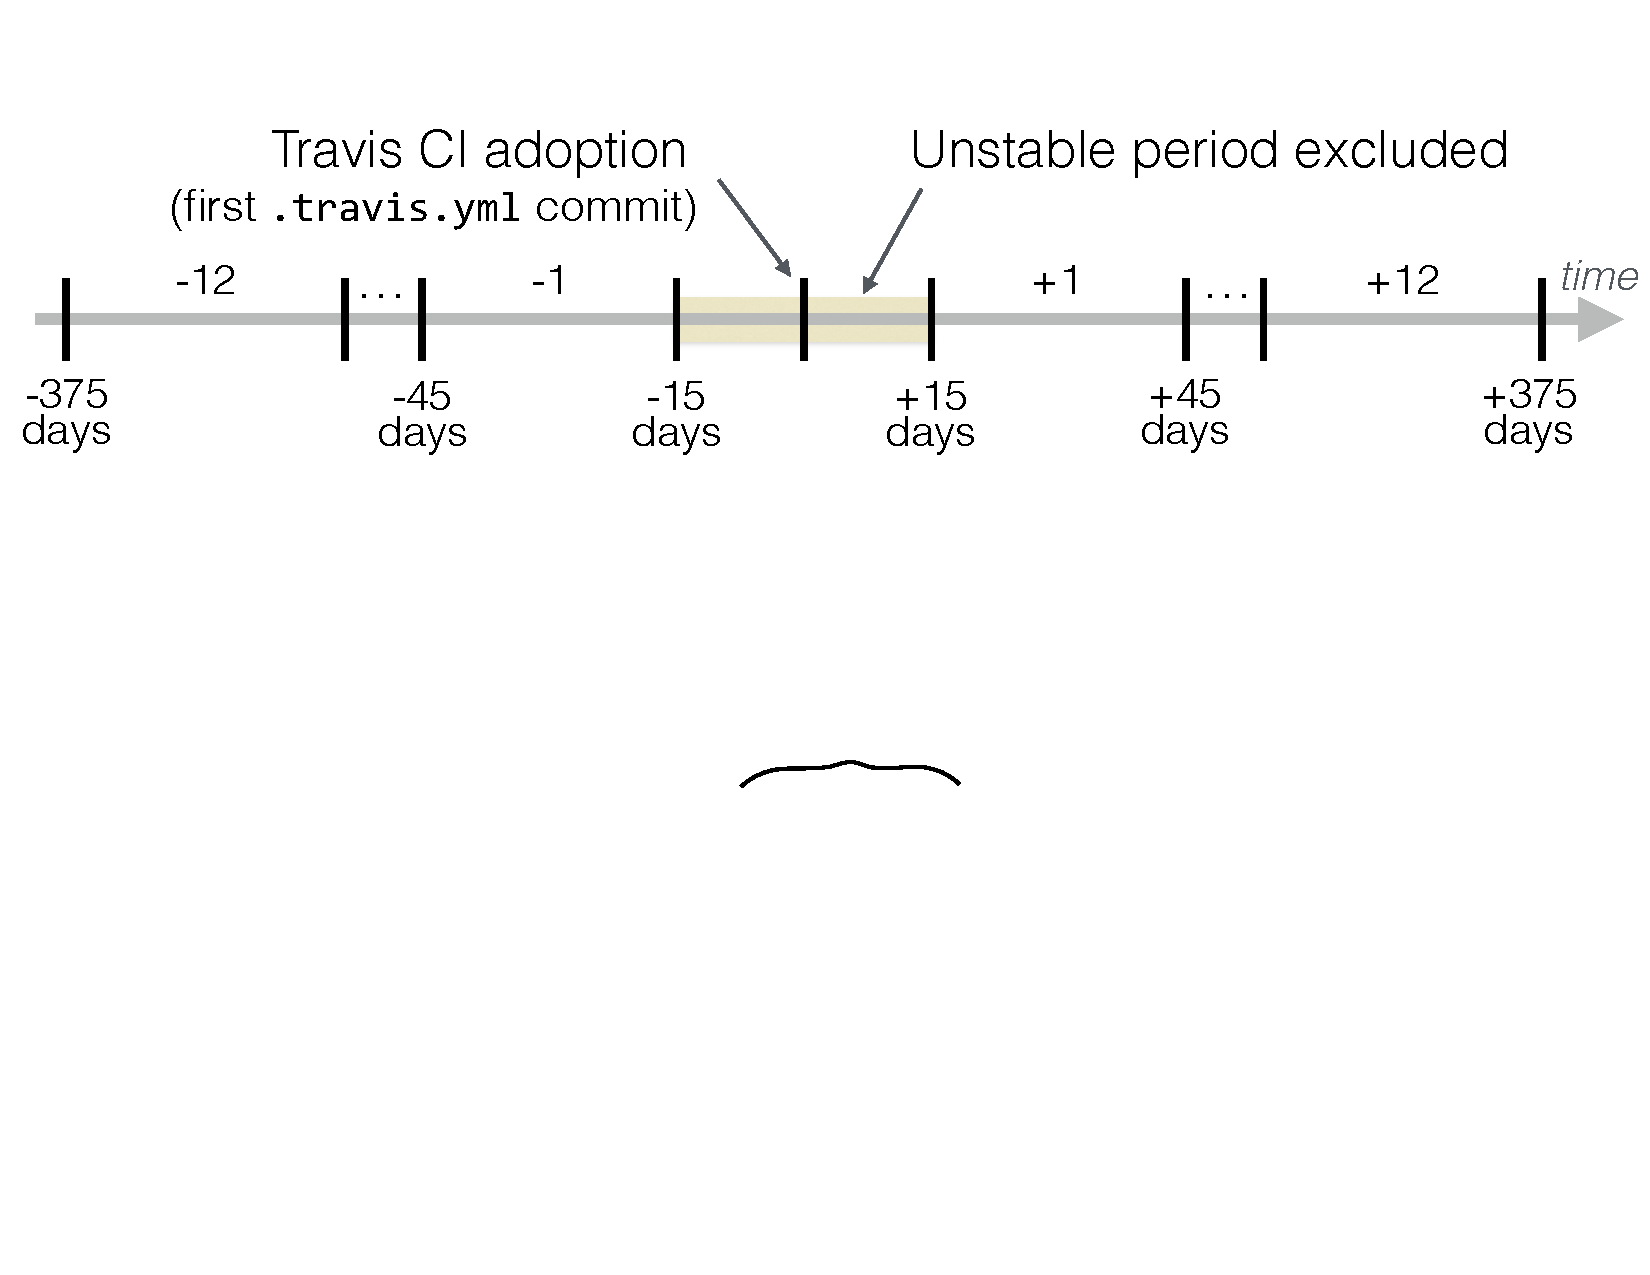
\includegraphics[width=\columnwidth, clip=true, trim=0 392 0 40]{figures/timeline.pdf}
	\caption{Overview of our time series assembly method.}%\vspace{-0.5cm}
	\label{fig:timeseries}
\end{figure}

\smallskip\noindent\emph{Time Series}

We proceeded to aggregate data about the different practices considered
in 30-day windows, 12 on each side, around the \Tvis adoption event
(Figure~\ref{fig:timeseries}).

During initial exploration, we observed that on several occasions \Tvi has 
been adopted as part of a larger restructuring effort, which lasted several days.
Examples include changing the build system from Ant to Gradle and, 
consequently, how project folders are organized; updating library 
dependencies; and restructured tests.
Based on this anecdotal evidence, we concluded that the activity immediately 
prior to and immediately following the introduction of \Tvis might not be 
representative of the project's overall trends.
Therefore, to limit the risk of bias due to extraordinary project activity in 
the transition period, we excluded one month of data centered around the 
adoption event in our quantitative analyses below.

\smallskip\noindent\emph{Measures}

We collected global and time-window-specific measures: 
\begin{itemize}

\item \textbf{total number of commits} in a project's history, as a proxy for 
project size / activity.

\item \textbf{total number of commit authors}, as a proxy for the size of a
project's community; commit authors include both core developers, who are
also committers, and external contributors, without ``write'' access, whose 
commits are merged in by the core developers.
Since it is common for open-source developers to contribute under different 
aliases (name-email tuples), \eg as a result of using different machines and 
changes in git settings over time, we first performed \emph{identity merging}.
We used heuristics that match first and last names, email prefixes, and email 
domains, cf.\ prior work~\cite{bird2006mining, vasilescu2015msrdata}, and
found an average of 1.15 (max 7) aliases per person in our dataset.

\item \textbf{project age} at the time of adopting \Tvis, in months, computed
since the earliest recorded commit.

\item \textbf{main programming language}, automatically computed by \GH
based on the contents of each repository and extensions of file names therein.

\item \textbf{number of non-merge commits}, \textbf{number of merge commits} 
per time window.
%, our measure of commit frequency.
Since git is a distributed version control system, developers can work locally,
in increments, before pushing their changes to \GH or opening a pull request.
E.g., a developer can choose to partition a large change into many smaller 
ones, and make multiple local commits to better manage the work.
This would not have any effect on CI runs, since CI is only triggered by \GH 
\emph{push} events, and events happening after (and including when) a pull 
request is opened.
%Pull requests are also a mechanism to isolate individual developers from 
%activity on the mainline.
Consequently, to study \emph{Commits To the \_Mainline\_ Every Day}
(Fowler's best practice), as opposed to potentially local git commits, we
distinguish between \emph{non-merge commits} and \emph{merge commits}
as a proxy.
We recognize non-merge commits as those having at most one parent, and
merge commits otherwise.

%\item  per time window.
%, as a proxy for how
%distributed a project's development is, over branches and forks.

\item \textbf{mean commit churn} for non-merge commits, per time window,
our measure of commit size.
Churn is computed as the total number of lines added plus the total number
of lines removed per commit (in git modified lines appear as first removed, 
then added), extracted from git logs.
The mean is computed over all non-merge commits commits in that time window.

\item \textbf{number of issues opened / closed}, \textbf{number of pull requests
opened / closed} per time window, extracted using the \GH API.

\item \textbf{mean pull request latency} per time window, in hours, computed 
as the difference between the timestamp when the PR was closed and that 
when it was opened.
The mean is computed over all PRs in that time window.
\end{itemize}

\bv{Add something about build logs and unit tests.}
%(i)~its history of commits, issues, and pull 
%requests using the \GH API; and 
%(ii)~its history of \Tvis builds and, for each
%build, all its job logs (a \Tvis build can be configured to run multiple jobs,
%one for each set of user-defined configuration options; each job run produces 
%a ``build log''), using the \Tvis API and the \textit{travis gem} Ruby library.  


\smallskip\noindent\emph{Filtering}

As a large fraction of projects on \GH are small and not highly 
active~\cite{gousios2014exploratory}, we filtered out projects that had not 
been consistently active during our 24-month observation period: we require
at least one commit on the main branch in each of the 24 time windows 
(in our sample only 2,595 projects, across 83 programming languages, satisfy 
this requirement).
Furthermore, our multivariate regression analysis below requires enough 
variance along each of the dimensions being modeled, thus we additionally
filter out programming languages not represented by at least 10 projects each.
The resulting dataset consists of 2,446 projects across 22 languages.

\bv{Talk about outlier removal}

\bv{Add dataset overview table}

% !TEX root = ../CI_Adoption.tex

\begin{table}[t] \centering
\small
  \caption{Examples for the outputs in terms of MAVEN, GRADLE and ANT
  \vspace{-0.2cm}
  }
  \label{log_example}

\begin{tabular}{ p{8cm}}
	\hline
	\\[-1.8ex]\hline
		\textbf{MAVEN}         \\
		\begin{tabular}[c]{@{}l@{}}
			\textit{-------------------------------------------------------}\\ 
			\textit{ T E S T S}\\ \textit{-------------------------------------------------------}\\ 
			\textit{Running org.sonar.ide.intellij.inspection.InspectionUtilsTest}\\ \textit{Tests run: 1, Failures: 0, Errors: 0, Skipped: 0, Time elapsed:}\\ \textit{0.202 sec}\\ 
			\textit{Results:}\\ 
			\textit{Tests run: 1, Failures: 0,Errors: 0, Skipped: 0}\end{tabular} \\  \hline
	
		\textbf{ANT}          \\
		\begin{tabular}[c]{@{}l@{}}
			\textit{{[}junit{]} Running limelight.BufferedImagePoolTest}\\ 
			\textit{{[}junit{]} Testsuite: limelight.BufferedImagePoolTest}\\ \textit{{[}junit{]} Tests run: 5, Failures: 0, Errors:0, Time elapsed: 0.143 sec}\end{tabular}                                                                                                                                                \\  \hline
		\textbf{GRADLE}          \\
		\begin{tabular}[c]{@{}l@{}}
			\textit{:test}\\ 
			\textit{...}\\ 
			\textit{1 test completed, 1 failed}\\
			\textit{:test FAILED}\\ 
			\textit{Total time: 3.8 secs}\end{tabular}      \\ \hline                                                                                                                                                                                                                                                
	\end{tabular}
\end{table}

\smallskip\noindent\emph{Number of Tests Executed per Build} 

We also parsed the \Tvis build logs and extracted information about the 
number of tests executed. % and the types of reasons causing builds to break.
%We provide more details next.
Each \Tvis build consists of at least one job, which corresponds to a particular
build and test environment (\eg jdk version, environment variables). 
Once the job is started, a log is generated, recording the detailed information
of the build lifecycle, including installation steps and output produced by the 
build managers. % scripts for testing. 
Table~\ref{log_example} shows fragments of the logs generated by the 
three widely used Java build tools, Maven, Ant, and Gradle. 
To investigate the evolution in testing practices across builds, we wrote a tool 
to analyze the logs and extract summary information about test executions.  
Since the relationship between builds and jobs is one-to-many, we use the 
maximum number of tests across jobs as the test count for the build. 



%We started by composing (using the \GH Search API) a list of candidate Java 
%projects that: (i)~were not very small (a large fraction of projects on \GH are 
%small and inactive~\cite{gousios2014exploratory}; we arbitrarily chose to ignore
%projects smaller than 500 kilobytes, using the \GH Search API's \emph{size} 
%parameter); and (ii)~were created no later than 2014-11-08. 
%The second criterion is a consequence of our data collection date (2016-05-01)
%and the ``sufficient history'' requirement. 
%Our statistical analysis, detailed below, assumes 9 months of history for each
%project both prior to and after adopting \Tvis; since we did not have access to
%data on when each project started using \Tvis at this stage, we conservatively
%chose the 2014-11-08 date, which allows 9*30*2 days of history from project 
%creation to 2016-05-01.
%This step resulted in a list of over 300,000 candidate Java projects.

%first and foremost, we should make sure our studied projects have sufficient history (e.g. 9*30 days) both before using Travis-CI and after using Travis-CI.  As the data were extracted from the inception until 2016-05-01, the projects selected should be created at least before 2014-11-08, so that there are at least 9*30*2 days from its creation to 2016-05-01. 
%From GitHub Search API, we first found over 300k Java projects created before 2014-11-08 and with $\geqslant 500$ kilobytes. 
%After consulting Travis-CI, we further identify projects that: 1) adopted Travis-CI; 2) at least 9 * 30 days from project creation to Travis-CI adoption; 3) at least 9 * 30 days from Travis-CI adoption to 2016-05-01. This filtering process left us 1566 projects.  
%For each project, we collect the whole history of commits, issues, and pull requests from GitHub API, and the history of Travis-CI builds and job logs from Travis-CI repository using the ruby library of \textit{travis gem}.  In addition to these publicly available data, we further gathered the information about the number of tests and types of errors during the Travis-CI run.

%Next, we used the \Tvis API to determine which of these projects:
%(i)~used \Tvis, and if yes, we recorded the date of the earliest build as the 
%adoption date; (ii)~had at least 9*30 days of history from project creation to 
%the adoption date, and from the adoption date to 2016-05-01, respectively. 
%This filtering process resulted in 1,566 projects.

%\smallskip\noindent\emph{Mainline commits:}
%
%Since git is a distributed version control system, developers can work locally,
%in increments, before pushing their changes to \GH or opening a pull request.
%E.g., a developer can choose to partition a large change into many smaller 
%ones, and make multiple local commits to better handle the work.
%This would not have any effect on CI runs, since CI is only triggered by \GH 
%push events, and events happening after (and including when) a pull request 
%is opened.
%%Pull requests are also a mechanism to isolate individual developers from 
%%activity on the mainline.
%Consequently, to study \emph{Commits To the \_Mainline\_ Every Day}
%(Fowler's best practice), as opposed to potentially local git commits, we
%distinguish between \emph{non-merge commits} and \emph{merge commits}
%as a proxy.
%We use  \texttt{\small git rev-list --all --merges} to recognize merge commits.

%Starting from RQ1 and RQ2 the practice being investigate should be �Commits To the Mainline Every Day�, but then you analyze git commits. Not surprisingly, commits do not increase. Why they should? The main reason of having many commits is the ability to partition a large change in many smaller ones and to better handle the work locally. What really matters for the CI are pushes and pull requests. Indeed, I would expect an increase of pushes/pull requests when CI is being adopted. Maybe a way to observe this is to actually analyze merge commits and see whether their frequency increases.
%Similar considerations apply for the size of code changes. Also, I�ve the feeling that such a size may strongly depend on the kind of activity being performed. For example, it could be that bug fixing correlates with small change size, whereas feature addition with larger ones. 

%\smallskip\noindent\emph{Bug fixing vs.\ other activities:} 
%
%The kind of activity being performed may confound commit size, \eg since one 
%can expect bug fix commits to be smaller than new feature implementations.
%We additionally annotate the non-merge commits as \emph{bug-fixing} or not, 
%by searching for typical patterns in commit 
%messages~\cite{mockus2000identifying}.\footnote{E.g., \verb$^(bug)?fix(es|s|ed|ing)?(bug)?([[:punct:]]|\\s+)$}
%Note that we don't enforce that commit messages that match our regular
%expressions also contain references to existing issue report numbers, in an
%attempt to be more robust to different issue trackers (indeed, not all projects 
%use \GH's issue tracker) and different project linking / commit message conventions.
%%
%%The "fix" heuristic without issue tracker links (looking for issue numbers and verifying they exist in the issue tracker) has the disadvantage that it will detect "false positives", i.e., commits made not in response to an open issue; plus the extra disadvantage that it will identify commit messages containing "suffix", for example.
%%
%%However, not all projects use GitHub's issue tracker, as we know and a reviewer pointed out. Also, the original intent, triggered by a review comment, was to distinguish between new features and bug fixes. We can say that the "fix" heuristic more closely accomplishes this by being robust to issue trackers and project linking conventions. The only downside I can think of is if people close open "feature request" issues from the issue tracker, using "fix" language.
%



%% !TEX root = CI_Adoption.tex

\begin{table}[t] \centering
\small
  \caption{Travis-CI build failure taxonomy
  \vspace{-0.2cm}
  }
  \label{error_types}

\begin{tabular}{ p{1.5cm}  p{2.5cm}  p{4cm} }
	
\hline 
\\[-1.8ex]\hline
Category & Description & Examples of textual patterns \\ \hline 
\emph{failed test} & tests were failed & tests failed, TestsFailedException, tests unsuccessful\\ \hline
\emph{skipped or pending test} & tests were skipped or set to be pending & skipped tests \\ \hline
\emph{missing file or dependency} & required files or dependencies are not available &  FileNotFoundException, no such file to load, is not installed \\ \hline
\emph{code quality} & the code failed to satisfy the code standards & line too long, missing whitespace around operator, too many pylint violations \\ \hline
\emph{compile error} &compilation errors happened & Compilation failed, syntax check failed, attributeError, parse error\\ \hline
\emph{execution error} &an error occurs during the execution of code & runtime error, execution failed, test errors, OutOfMemoryError\\ \hline
\emph{time out} & the build could not be completed within the required time&“test run exceeded * minutes”, “..took longer than”, command time-out \\ \hline 
\emph{other} &other infrequent errors are included in this type & warnings on documentation, Aborted due to warnings, The remote end hung up unexpectedly \\
\hline

\end{tabular}

\end{table}



%\smallskip\noindent\emph{Error classification for failed builds:}
%
%\Tvis marks a build as \textit{failed} if at least one of its jobs not explicitly 
%labeled as \emph{allowed to fail} in the project's CI configuration 
%file\footnote{\url{https://docs.travis-ci.com/user/customizing-the-build/#Rows-that-are-Allowed-to-Fail}} failed.
%Therefore, to understand why \Tvis builds failed, we proceed to find out 
%what happened in the jobs. 
%We first manually reviewed a set of failed jobs to recognize what kinds of 
%failures occur and whether there are any corresponding textual patterns in 
%the logs.
%Then, we extracted a set of mapping rules to classify these patterns into 
%categories.
%We proceeded iteratively by inspecting more randomly selected failed jobs
%and gradually refining our classification scheme, until reaching saturation. 
%%To mitigate the risk of bias arising from missing and incorrect classification, 
%%we augmented the manual reviewing rates to improve our classification 
%%rules and remove spurious classification as much as possible. 
%%The classification scheme evolved during this process, and was gradually 
%%refined to cover more textual patterns. 
%In the end, we identified 8 categories of reasons for build failures, 
%as summarized in Table~\ref{error_types}. 
%%a group of mapping rules to classify the errors into 8 types, as shown 
%
%Next, we implemented tools for automatic classification. 
%The detailed process comprises the following steps:
%
%\noindent 1)~\emph{Failure Location}. 
%We first recognized failed jobs with \textit{non-allow-failure} attributes, which 
%result in the build's final \textit{failed} state. 
%Then, we attempted to locate the command which caused the breakdown 
%in the log file, as the command which exited with a non-zero value.
%The log entry for this command usually provided detailed information about 
%the fatal errors that occurred. 
%If such commands were not recorded in the log file, we expanded the search 
%scope to the \textit{script} phase and the \textit{after script} phase of the 
%build log, as per \Tvis build lifecycle.\footnote{\url{https://docs.travis-ci.com/user/customizing-the-build/#The-Build-Lifecycle}}
%Note that if errors occur in the \emph{before script} phase of the build, the 
%job is automatically marked as \textit{errored} and stops immediately. 
%Only if the \textit{script} phase returns a non-zero exit code, or the \textit{after 
%script} phase times out, then the job is marked as \textit{failed}. 
%Therefore, we first check if there is a time-out error in \textit{after script}. 
%If not, then it's likely that the errors in the \textit{script} phase caused the 
%build to break. 
%
%\noindent 2)~\emph{Log Parsing \& Tagging}. 
%After extracting the log fragment describing the errors, we 
%used textual pattern matching for classification. 
%%
%%\noindent 3)~\emph{Tagging}. 
%%We tagged the extracted textual patterns with a subset of the defined 8 error 
%%types. 
%Note the one-to-many relationship between jobs and failure types. 
%E.g., if a job had both failed tests and skipped tests, it is tagged 
%with both ``failed test'' and ``skipped or pending test'' error types.


%\textit{Distinguishing the bugs introduced before CI adoption and the bugs introduced after CI adoption}: 
%We suppose that the defects before and after introducing Travis-CI are different. To verify this, we use the SZZ algorithm to gather bug data, and divide them into two groups ( \ie bugs introduced before Travis-C and bugs introduced after Travis-CI ).
%In GitHub, when a bug is reported, an issue will be created to track this bug, and subsequently a set of commits occur for bug fixing. 
%We decide whether a issue is a \textit{fix issue} based on the constrains that 1) the issue has been taged as a bug (with labels like \textit{bug}, \textit{defect}, \textit{fault}); 2) the issue has at least one commit with source file modification to fix this bug. To do this, We first analyze the commit messages to recognize its corresponding issue based on the special textual patterns (\eg fix \textit{issue\_id}, close \textit{issue\_id}, gh-\textit{issue\_id}), and then check if this issue has bug tag. If yes, we will use git diff to find the change details (\ie changed files and lines), and further check if the commit has changed source files.
%After the above conditions checking, we identify fix issues and the corresponding fix commits. The lines changed in fix commits are targeted to fix the bug. Using \textit{git blame}, we can locate which commit last added or modified these lines. We consider this commit as a buggy commit as it introduced bug. 
%As we know, a fix issue will only be triggered by the bug introduced before the issue is opened. Therefore, a necessary condition for filtering is that the buggy commit must have been pushed before the bug being reported (\ie issue being created), otherwise, this buggy commit should not be implicated.
%With above process, the bugs can be divided into two groups based on when the bugs were introduced (\ie buggy commit time) and when the project started using Travis-C. For each group, we gathered the bug logs from the fix issues and fix commits, and then built word cloud to analyze the differences between them.

%\subsection{Overview of the Data Set}
\subsection{Additional RQ-Specific Filtering}
\label{sec:dd}

% !TEX root = CI_Adoption.tex



\begin{table}[]
	\centering
	\caption{Summary statistics for 1566 studied projects}
	\label{projs_summary}
	\begin{tabular}{ p{1.2cm} p{0.7cm} p{0.7cm} p{0.7cm} p{0.7cm} p{0.7cm} p{0.7cm}}
		\hline
		Statistic       & Min            & 1st Qu.        & Median          & Mean           & 3rd Qu.        & Max             \\ \hline
		
		created\_at     & 2008/6/6 & 2011/8/8  & 2012/7/30 & 2012/6/27 & 2013/6/6  & 2014/11/7 \\
		size            & 500            & 1594           & 6006            & 40460          & 26980          & 2433000         \\
		
		\# stars        & 0              & 6              & 33.5            & 344.1          & 180.8          & 18480           \\
		\# forks        & 0              & 4              & 18              & 133.2          & 74             & 7247            \\
		
		\# commits      & 5              & 184.2          & 412             & 1385           & 1085           & 118000          \\
		\# issues       & 0              & 2              & 20              & 125.9          & 89.75          & 10330           \\
		
		\# PRs & 0              & 2              & 14              & 97.68          & 64             & 7715            \\
		\# builds       & 1              & 39             & 99.5            & 347            & 278            & 16700          
	\end{tabular}
\end{table}


%Our study makes use of a large-scale data set collected from the selected 1566 java projects. 
Table~\ref{projs_summary} contains descriptive statistics for the selected 
1,566 Java projects that adopted \Tvis. 
We note an average number of 347 builds per project. 
We further census the builds in terms of the triggering event type and final 
state (Table~\ref{builds_count}). 
Out of 541,959 builds total in our data set, 68\% came from push commits 
and 32\% from pull requests (PRs). 
Of these builds, 67.1\% passed, 18.6\% failed, and the others errored or were canceled. 
In addition, Table~\ref{count_info} lists statistics for \#Commits, \#Issues, 
and \#PRs before and after adopting \Tvis, respectively. 
We can preliminarily see that there are fewer commits 
after adopting CI, but more issues and PRs.
From the summary statistics, we found there are large variances between 
projects in terms of each attribute (Table~\ref{projs_summary}).
For example, 18\% of projects have no \GH issues;
% a value of \#issues equal to 0, as they 
%haven't used \GH issue tracking yet. 
when studying the evolution of issue reporting practices, these projects without 
issues may bias our conclusions. 
As a result, to avoid too many zeros in our subsequent time series analysis, 
we did more data filtering for each RQ individually, as follows.
%based on different conditions, 


For RQ1 and RQ2, we study code churn and commit frequency. 
To reduce potential bias due to data sparsity (since we aggregate data at 
monthly intervals; see Section~\ref{sec:tsa}), we discard projects having 
fewer than 500 total non-merge commits (arbitrarily chosen).
%In our data set, 8.9\% of commits are merge commits. 
%First, we remove these merge commits, to avoid double counting and since 
%they were automatically generated. 
%Then, we further filter the projects based on the number of non-merge commits,
%to reduce potential bias due to data sparsity (since we aggregate data at 
%monthly intervals), and discard projects with less than 500 total non-merge 
%commits.
%%We Each project should have at least 500 nonmerge commits. 
This restricts the data set to 567 projects, with a 
total of 1,629,090 non-merge commits (of them, 274,410 are fix commits) 
and 157,976 merge commits.

For RQ3, we only selected projects with at least 100 issues for similar sparsity 
avoidance reasons. 
The resulting filtered data set contains 293 projects (143,573 \GH issues total).

For RQ4, we investigate changes in \#tests per build.
As introduced above, we collected \#tests from build logs. 
First we filtered the projects based on the number of builds
(lower bound arbitrarily set at 100), leaving 736 projects. 
%Each projects should have at least 100 builds. This selection left us 736 projects. 
Furthermore, during the collection of \#tests, we found (and subsequently
filtered out) 219 projects that did not execute any tests as part of their \Tvis 
builds, and additional 267 projects that tested scarcely (\ie we kept 
projects for which at least 90\% builds executed at least one test). 
%We just removed these projects as they didn't have \# test values. 
In the end, 250 projects remained in the filtered RQ4 data set.
%Among the other projects, 250 of them have more than 90\% builds with at least one test. Here, we only consider these 250 projects with high coverage of testing ( \textgreater{ 90\%} ).

\subsection{Time Series Analysis Method}
\label{sec:tsa}

We use data visualization and statistical modeling to discover 
longitudinal patterns indicative of CI adoption effects on development practices.
As one of our contributions, we introduce the statistical modeling 
framework of \emph{regression discontinuity design}~\cite{imbens2008regression} 
to assess the existence and extent of a longitudinal effect of CI adoption on 
development practices.

To evaluate the effect of a treatment, \eg new drug on a disease progression, 
randomized experimental trials are conducted, 
in which the experimental 
cohort is randomly split into a treatment group, \ie those given the treatment, and 
a control group, \ie those not given the treatment. 
Then, the effect is evaluated based on the difference in disease progression 
between the two groups.
In the absence of randomized trials, as is the case with trace data in 
empirical software engineering, weaker techniques which make 
additional assumptions, \eg quasi-experiments, are employed.

Regression discontinuity design (RDD)~\cite{imbens2008regression} is an example of such a technique, 
used for modeling the extent of a discontinuity of a function between its values 
at points just before and just after a given intervention. 
RDD is based on the assumption that in the absence of the intervention, the 
trend of the function would be continuous in the same way as prior to it.
Fig.~\ref{RDDIllustration} illustrates a discontinuity, and the RDD approach, in a nutshell, aims to uncover the 
 different regression lines before and after the discontinuity.

There are a number of different formalizations of RDD, most prominently 
sharp RDD and fuzzy RDD~\cite{imbens2008regression}.
%Each, in turn, can be implemented in a variety of ways.
To model the effect of CI adoption on developer practices, here we chose one implementation
of the simpler, sharp RDD approach: linear regression with an interaction term.
We summarize our approach next, following the description by Imbens and 
Lemieux~\cite{imbens2008regression}, and refer to Figure~\ref{RDDIllustration}.
Let $Y$ be the outcome variable in which we are looking for a discontinuity, 
\eg change in commit churn per month before vs after CI adoption, let $X$ be the temporal variable containing the 
time of intervention, and let $c$ be the time point at which the intervention, \eg CI adoption, has occurred.
Then, an RDD model for points $x_i$ in equal intervals $h$ on each side of 
$c$, $c-h \le x_i \le c+h$, is given by:

\[y_i \ = \alpha + \beta(x_i-c) + \gamma w_i + \delta(x_i-c)w_i + \epsilon_i,\]

\noindent where $w_i = (x_i \geq c)$, \ie $w_i$ is 1 if point $x_i$ is included in 
the treatment group (\eg after CI adoption), and 0 if it is before the treatment.
In fact, this model encapsulates two separate regressions.
For points before the treatment, the resulting regression line has a slope of 
$\beta$, and after the treatment $\beta + \delta$.
The size of the effect of the treatment is the difference between the two 
regression values of $y_i$ evaluated at $x=c$, and can be seen to be equal 
to $\gamma$.
For example, in Fig.~\ref{RDDIllustration}, the treatment effect ($\gamma$) is negative, and there is an interaction effect ($\delta \neq 0$) which changes the slope of the regression after the treatment.
A critical assumption for RDD is that but for the treatment, all other variables remain steady, before, during, and after the treatment.

For each project, we use an RDD model implemented as the above 
double linear regression, on data centered at the time of CI adoption, and 
having equal number of points on each side.
Solving the regression gives us the coefficients, which if significant, can help us reason about the treatment and its effects, if any.
We report on the models having significant coefficients in the regressions ($<0.05$). Our successful models had an $R^2$ of at least $0.65$. 



\begin{figure}[t]
	\centering
	\includegraphics[width=0.4\textwidth, clip=true, trim=0 15 15 50]{RDD_plot.png}
	\caption{RDD illustration.}\vspace{-0.5cm}
	\label{RDDIllustration}
\end{figure}



\section{Results and Discussion}

We sought to study how different software development practices evolve around the time of CI adoption and the period after the adoption.

\subsection{RQ1: Changes in Code Churn Practices}

The first development practice we examine is code churn.
The data consists of 567 projects, each with at least 500 nonmerge commits.

\noindent \underline{Exploratory Study} To explore general trends over time, we first look at code churn in months leading up to CI adoption.
Fig.~\ref{Fig:CodeChurnBefore} shows a boxplot of per-project median code churn for each of nine consecutive 30-day time intervals before CI adoption.
The verical line in each boxplot is the median value of all per-project median, and the black dot is their average value.
We observe that for most part, the medians dance around 
10 and 12 lines of code churn per period, and the averages between 16 and 18 lines, with large variance and no obvious trend. The 30-day interval just before CI adoption seems to stand out and is higher than the rest.

We look to the other side of the adoption point next. Fig.~\ref{Fig:CodeChurnBefore} shows a boxplot of per-project median code churn for each of nine consecutive 30-day time intervals following CI adoption.
Here, the story the boxplots are telling looks different. There is an apparent, downward trend in both the medians and averages, the former drop from 13 down to 7-8 lines of code and the average down to 15 lines of code.
The 30- and 60-day intervals just after the adoption point seem to be higher than the rest, and together with the 30-day interval just before adoption of CI seem to form a peak of increased code churn.
The trend in the medians is significant statistically (which test?, p-val = 0.0014).
Not considering the peak behavior in code churn around CI adoption time, we observe a 30\% reduction in the amounts of code churn.


\begin{figure}[!t]
\centering
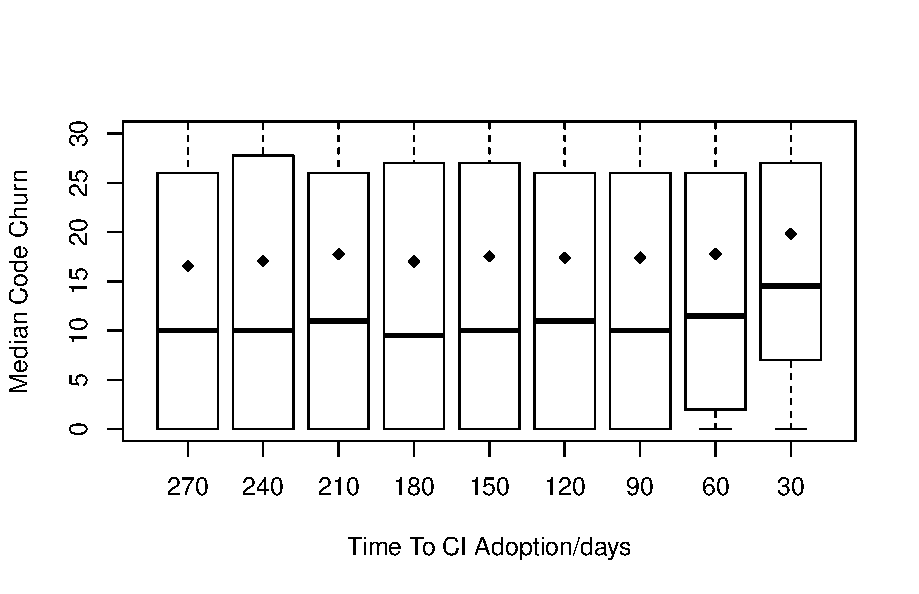
\includegraphics[width=0.5\textwidth]{churn_before.pdf}
\caption{The Code churn before CI adoption}
\label{Fig:CodeChurnBefore}
\end{figure}



\begin{figure}[!t]
\centering
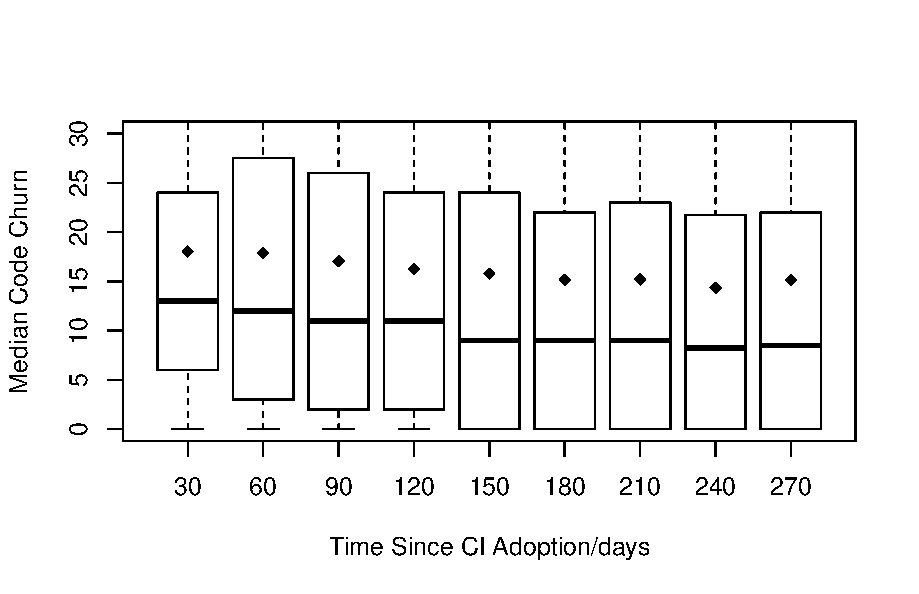
\includegraphics[width=0.5\textwidth]{churn_after.pdf}
\caption{The Code churn after CI adoption}
\label{Fig:CodeChurnAfter}
\end{figure}

\noindent \underline{Modeling Study} 


Table 1: Summary of all models

Table 2: Projects with negative trends after CI

\noindent \underline{Discussion}
The increased code churn on both sides near the CI adoption time is arguably in line with expectations that more maintanance work may be going on in preparation for the transition to CI, and that the projects go through some adjustment/cleanup period right after.

\subsection{RQ2: Trends in Testing}




Fig 3: Box plots of fraction of builds with tests or unit tests per pull request, per unit time period, one for each time point, each point an aggregate of all projects

Fig 4


\subsection{RQ3: Changes in Issues}

Fig 5: Box plots of \# issues per unit time period, one for each time point, each point an aggregate of all projects



% !TEX root = CI_Adoption.tex
\section{Related Work}
\label{sec:rw}
Adoption and impact of continuous integration have attracted \as{limited/extensive} attention from the research community. Already in 2003 based on the studies of FreeBSD and Mozilla Holck and J{\o}rgensen have observed that continuous integration, interpreted as distributed development and obligation to integrate one's own contributions, is capable of replacing traditional software engineering coordination mechanisms~\cite{HolckJ03}.  
Deshpande and Riehle have studied adoption of continuous integration based on Ohloh.net data~\cite{Deshpande2008}. Assuming that the use of continuous integration reduces the size of commits, they have studied the size of commits in 5122 projects and, since no commit size reduction has been observed, they have concluded that continuous integration has not been used. Their observations might have been affected by lack of actual relation between presence of continuous integration and commit size, aggregation effect of considering the average commit size over different projects as well as the period studied (January 1990--December 2006). 

Ease of use of the Travis-CI~\cite{TravisCI} continuous integration system led to its popularity on GitHub and triggered a series of research studies~\cite{era14,VasilescuYWDF15,yue2015wait,BellerGZ16,Hilton2016,Yu2016}.\as{To be continued. Maybe Bogdan can write about his own work.}

Industrial adoption of continuous integration systems has been recently studied in several papers~\cite{Leppanen2015,Laukkanen2015Agile,Debbiche2014,Stahl2014ICSEComp,Stahl2014JSS} and is a subject of the recent survey by Eck, Uebernickel and Brenner~\cite{EckUB14}. However, this line of work is based on interviews rather than on analysis of the development data.

\as{Miller~\cite{Miller} discusses build breaks, is this relevant?}
\as{Van der Storm discusses backtracking as a way of addressing build failures~\cite{Storm2008}.}
\as{Laukannen and M\"{a}ntyl\"{a} have surveyed three papers discussing the impact of the build waiting times. Some of the consequences of the long/short build waiting times are related to CI~\cite{Laukkanen2015RCSE}.}


\section{Conclusion}

\begin{figure}[!t]
\centering
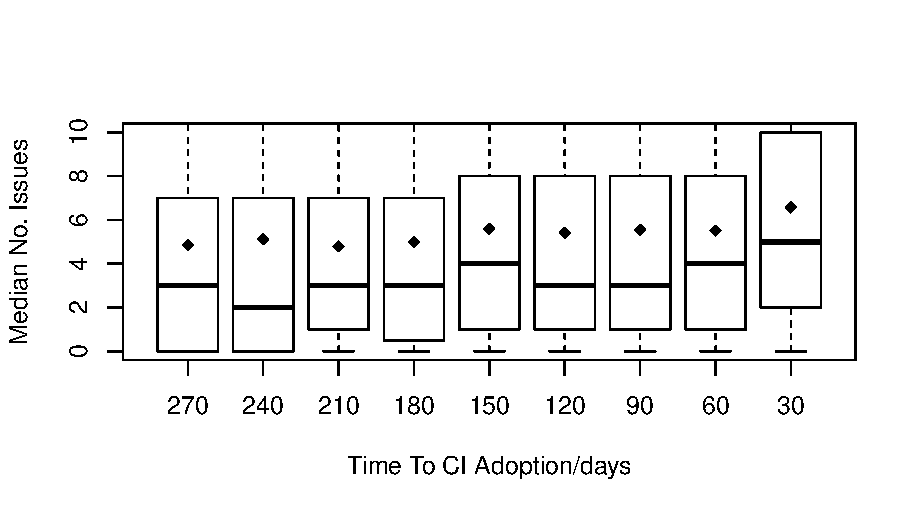
\includegraphics[width=0.5\textwidth]{issues_before.pdf}
\caption{Median number of issues before CI adoption}
\label{Fig:IssuesBefore}
\end{figure}


\begin{figure}[!t]
\centering
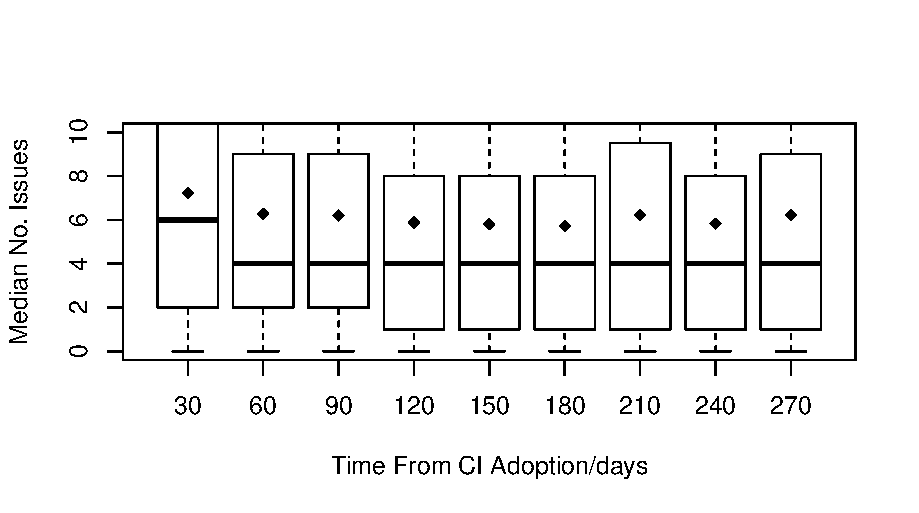
\includegraphics[width=0.5\textwidth]{issues_after.pdf}
\caption{Median number of issues after CI adoption}
\label{Fig:IssuesAfter}
\end{figure}


\begin{figure}[!t]
\centering
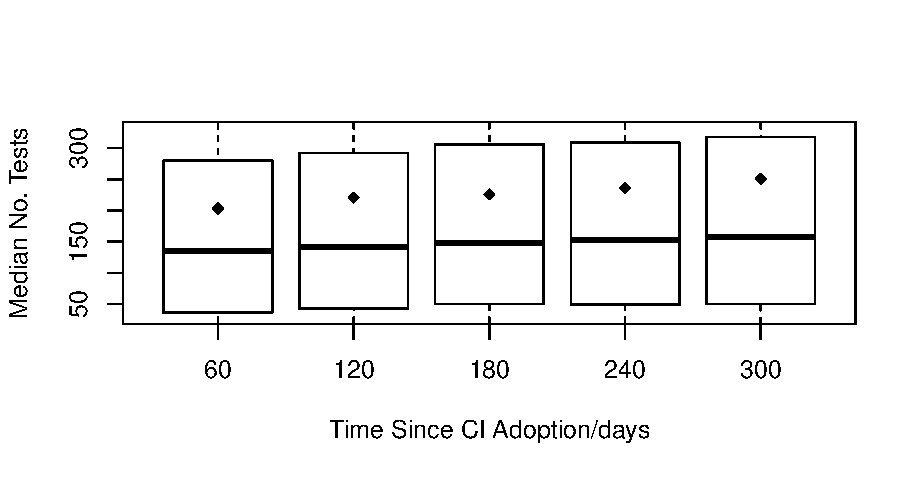
\includegraphics[width=0.5\textwidth]{tests.pdf}
\caption{Unit tests per build following CI adoption}
\label{Fig:Tests}
\end{figure}

\section{Threats to Validity}

\begin{figure}[!t]
\centering
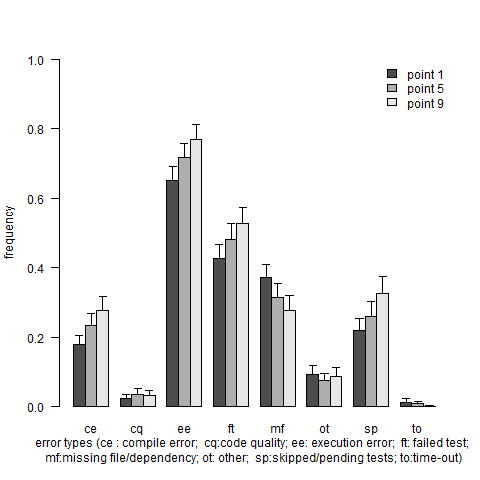
\includegraphics[width=0.5\textwidth]{plot_together.png}
\caption{Evolution of Error Types Since CI Adoption}
\label{Fig:BugTypes}
\end{figure}


\bibliographystyle{IEEEtran}
\bibliography{references}

\end{document}